\documentclass[border=1pt]{standalone}
\usepackage{fontspec}
\usepackage[dvipsnames,svgnames]{xcolor} % Extended color support
\usepackage{tikz}
\usepackage{pgfplots}
\usepackage{amsmath}
\usepackage{amssymb}
\usepackage{mathtools}
\usepackage{unicode-math}
\usepackage{graphicx}
\usepackage{microtype}
\usepackage{enumitem}

\pgfplotsset{
  compat=1.18
}

%\setmainfont{Libertinus Sans}
%\setsansfont{Libertinus Sans}
%\setmonofont{Libertinus Mono}
%\setmathfont{Libertinus Math}

\setmainfont{Noto Sans}
\setsansfont{Noto Sans}
\setmonofont{Noto Sans Mono}
\setmathfont[
  Path=fonts/,
  Extension=.ttf
]{NotoSansMath-Regular}

\usetikzlibrary{
  calc,
  positioning,
  intersections,
  through,
  angles,
  quotes,
  arrows.meta,
  patterns,
  decorations.pathreplacing,
  decorations.markings,
  decorations.text,
  shapes,
  shapes.geometric,
  matrix,
  fit,
  backgrounds,
  fadings
}

\begin{document}
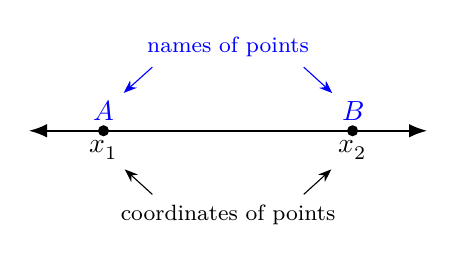
\begin{tikzpicture}[>=Latex]
  \tikzset{
    dimline/.style={
      arrows={Bar[length=0pt,width=14pt]}-{Bar[length=0pt,width=14pt]}
    },
    dot ends/.style={
      {Circle[length=2pt]}-{Circle[length=2pt]}
    },
    %    every path/.style={thick},
    % every node/.style={font=\large}
  }
\coordinate (a) at (0,0);
\coordinate (b) at (90pt,0);
\draw[thick, <->] ($(a)!-0.3!(b)$)--($(a)!1.3!(b)$)
node[midway,below=23pt, name=coord] {\footnotesize coordinates of points}
node[midway,above=23pt, name=names, color=blue] {\footnotesize names of points};

\fill[] (a) circle (2pt) node[below, name=x1] {$x_1$}
node[above, name=anode, color=blue] {$A$};
\fill[] (b) circle (2pt) node[below, name=x2] {$x_2$}
node[above, name=bnode, color=blue] {$B$};

\draw[-{Stealth}] (coord.165)--(x1);
\draw[-{Stealth}] (coord.15)--(x2);

\draw[-{Stealth}, draw=blue] (names.-165)--(anode);
\draw[-{Stealth}, draw=blue] (names.-15)--(bnode);


\end{tikzpicture}

\end{document}
